%%%%%%%%%%%%%%%%%%%%%%%%%%%%% Define Article %%%%%%%%%%%%%%%%%%%%%%%%%%%%%%%%%%
\documentclass{article}
%%%%%%%%%%%%%%%%%%%%%%%%%%%%%%%%%%%%%%%%%%%%%%%%%%%%%%%%%%%%%%%%%%%%%%%%%%%%%%%

%%%%%%%%%%%%%%%%%%%%%%%%%%%%% Using Packages %%%%%%%%%%%%%%%%%%%%%%%%%%%%%%%%%%
\usepackage{geometry}
\usepackage{graphicx}
\usepackage{amssymb}
\usepackage{amsmath}
\usepackage{amsthm}
\usepackage{empheq}
\usepackage{mdframed}
\usepackage{booktabs}
\usepackage{lipsum}
\usepackage{graphicx}
\usepackage{color}
\usepackage{psfrag}
\usepackage{pgfplots}
\usepackage{bm}
\usepackage{hyperref}
\usepackage[T1]{fontenc}
\usepackage[utf8]{inputenc}
%%%%%%%%%%%%%%%%%%%%%%%%%%%%%%%%%%%%%%%%%%%%%%%%%%%%%%%%%%%%%%%%%%%%%%%%%%%%%%%

% Other Settings

%%%%%%%%%%%%%%%%%%%%%%%%%% Page Setting %%%%%%%%%%%%%%%%%%%%%%%%%%%%%%%%%%%%%%%
\geometry{a4paper}

%%%%%%%%%%%%%%%%%%%%%%%%%% Define some useful colors %%%%%%%%%%%%%%%%%%%%%%%%%%
\definecolor{ocre}{RGB}{243,102,25}
\definecolor{mygray}{RGB}{243,243,244}
\definecolor{deepGreen}{RGB}{26,111,0}
\definecolor{shallowGreen}{RGB}{235,255,255}
\definecolor{deepBlue}{RGB}{61,124,222}
\definecolor{shallowBlue}{RGB}{235,249,255}
\definecolor{Red}{RGB}{240,20,10}
%%%%%%%%%%%%%%%%%%%%%%%%%%%%%%%%%%%%%%%%%%%%%%%%%%%%%%%%%%%%%%%%%%%%%%%%%%%%%%%

%%%%%%%%%%%%%%%%%%%%%%%%%% Define an orangebox command %%%%%%%%%%%%%%%%%%%%%%%%
\newcommand\orangebox[1]{\fcolorbox{ocre}{mygray}{\hspace{1em}#1\hspace{1em}}}
%%%%%%%%%%%%%%%%%%%%%%%%%%%%%%%%%%%%%%%%%%%%%%%%%%%%%%%%%%%%%%%%%%%%%%%%%%%%%%%

%%%%%%%%%%%%%%%%%%%%%%%%%%%% English Environments %%%%%%%%%%%%%%%%%%%%%%%%%%%%%
\newtheoremstyle{mytheoremstyle}{3pt}{3pt}{\normalfont}{0cm}{\rmfamily\bfseries}{}{1em}{{\color{black}\thmname{#1}~\thmnumber{#2}}\thmnote{\,--\,#3}}
\newtheoremstyle{myproblemstyle}{3pt}{3pt}{\normalfont}{0cm}{\rmfamily\bfseries}{}{1em}{{\color{black}\thmname{#1}~\thmnumber{#2}}\thmnote{\,--\,#3}}
\theoremstyle{mytheoremstyle}
\newmdtheoremenv[linewidth=1pt,backgroundcolor=shallowGreen,linecolor=deepGreen,leftmargin=0pt,innerleftmargin=20pt,innerrightmargin=20pt,]{theorem}{Theorem}[section]
\theoremstyle{mytheoremstyle}
\newmdtheoremenv[linewidth=1pt,backgroundcolor=shallowBlue,linecolor=deepBlue,leftmargin=0pt,innerleftmargin=20pt,innerrightmargin=20pt,]{definition}{Definition}[section]
\theoremstyle{myproblemstyle}
\newmdtheoremenv[linecolor=black,leftmargin=0pt,innerleftmargin=10pt,innerrightmargin=10pt,]{problem}{Problem}[section]
%%%%%%%%%%%%%%%%%%%%%%%%%%%%%%%%%%%%%%%%%%%%%%%%%%%%%%%%%%%%%%%%%%%%%%%%%%%%%%%

%%%%%%%%%%%%%%%%%%%%%%%%%%%%%%% Plotting Settings %%%%%%%%%%%%%%%%%%%%%%%%%%%%%
\usepgfplotslibrary{colorbrewer}
\pgfplotsset{width=8cm,compat=1.9}
%%%%%%%%%%%%%%%%%%%%%%%%%%%%%%%%%%%%%%%%%%%%%%%%%%%%%%%%%%%%%%%%%%%%%%%%%%%%%%%

%%%%%%%%%%%%%%%%%%%%%%%%%%%%%%% Title & Author %%%%%%%%%%%%%%%%%%%%%%%%%%%%%%%%
\title{An Investigation in Cartesian Planes}{
\author{Tushar Maharana \thanks{Existence\#6673 (Discord user)}}
%%%%%%%%%%%%%%%%%%%%%%%%%%%%%%%%%%%%%%%%%%%%%%%%%%%%%%%%%%%%%%%%%%%%%%%%%%%%%%%

\begin{document}
    \maketitle
    We can make equations that represent a line on the Cartesian plane.
    \begin{equation}
        x + y = 0
    \end{equation}
    \begin{align}
    \begin{tikzpicture}
        \begin{axis}[xmin=-5, xmax=5, ymin=-5, ymax=5, axis x line=middle, axis y line=middle]
            \addplot[color=deepBlue] {-x};
        \end{axis}
    \end{tikzpicture}
    \end{align}
    These are also called linear equations.\\ 
    Let's say we do it the other way around and make a equation, who's solution is what we choose.
    We want a equation, whose solution is

    \begin{equation}
        x = 1 , y = 0
    \end{equation} 
    Let's try adding the equations,
    so,
    \begin{equation}
        x + y = 1 + 0
    \end{equation}
    \begin{equation}
        x + y = 1
    \end{equation}
    Let's verify it graphically, \\
    \begin{align}
    \begin{tikzpicture}
        \begin{axis}[xmin=-5, xmax=5, ymin=-5, ymax=5, axis x line=middle, axis y line=middle]
            \addplot[color=deepBlue] {1-x};
            \addplot coordinates {(1,0)};
        \end{axis}
    \end{tikzpicture}
    \end{align}
    Yay! We did it!\\
    
    Now what about 2 solutions equations?\\

    Umm, I think these equation are also called Quadratic Equations. \\
    Anyway,
    Let's say the required points are
    \begin{align}
        x_{1} = 1 \\
        y_{1} = 0 \\
        x_{2} = 2 \\
        y_{2} = 0
    \end{align}
    Now to create the equation. Let's first make a equation for each point first.
    \begin{align}
        x + y = 1 + 0 \\
        x + y = 1
    \end{align}
    \begin{align}
        x + y = 2 + 0 \\
        x + y = 2 
    \end{align}
    Upon further rearrangement, \\
    \begin{align}
        x + y - 1 = 0 \\
        x + y - 2 = 0 
    \end{align}
    Let's use the factor theorem to make a equation
    \begin{align}
        (x + y - 1)(x + y - 2) = 0 \\
        x^2 + xy -2x + xy + y^2 -2y -x -y + 2 = 0 \\
        x^2 + y^2 + 2xy - 3 (x + y) + 2 = 0
    \end{align}
    We have a equation now!
    Let's verfiy using a graph.
    \begin{align}
    \begin{tikzpicture}
        \begin{axis}[xmin=-5, xmax=5, ymin=-5, ymax=5, axis x line=middle, axis y line=middle]
            \addplot[color=deepBlue] {1-x};
            \addplot[color=deepBlue] {2-x};
            \addplot coordinates {(1,0)(2,0)};
        \end{axis}
    \end{tikzpicture}
    \end{align}
    Damn, that's satisfying! Do you know what's even more satisfying? There are infinite solutions to our question.\\
    Let's try finding the other solutions. \\ \\ 
    This is the factored form of the equation we had obtained.
    \begin{align}
        (x + y - 1)(x + y - 2) = 0 
    \end{align}
    If we manipulate them
    and take y as the function we get,
    \begin{align}
        f(x)=(1-x)(2-x)\\
        f(x)=2-x-2x+x^2 \\
        f(x)=x^2-3x+2
    \end{align}
    Let's graph this one and try again.
    \begin{align}
        \begin{tikzpicture}
            \begin{axis}[xmin=-5, xmax=5, ymin=-5, ymax=5, axis x line=middle, axis y line=middle]
                \addplot[color=deepBlue] {x^2-3*x+2};
                \addplot coordinates {(1,0)(2,0)};
            \end{axis}
        \end{tikzpicture}
        \end{align}
    We found another equation, I am sure that there are many more! But I haven't found another one yet. But if you find one email me at \href{mailto:tusharmaharana44676@gmail.com}{tusharmaharana44676@gmail.com}.
    \section{Existence\#6673}
    Existence told me about the general form of these equations.

    Any equation having the solutions $1$ and $2$ ($y = 0$) is in the form of,
    \begin{align}
        f(x)=ax^n(x-1)(x-2)
    \end{align}
    We just got a infinite supply of these equations! \\
    Let's create four of them and graph them!
    \begin{align}
        \color{ocre}{f(x)=(x-1)(x-2) , a = 1 , n = 0} \\
        \color{Red}{f(x)=2x(x-1)(x-2) , a = 2 , n = 1}\\
        \color{deepGreen}{f(x)=3(x^2)(x-1)(x-1) , a = 3 , n = 2}\\
        \color{deepBlue}{f(x)=4(x^3)(x-1)(x) , a = 4 , n = 3}
    \end{align}
    \begin{align}
    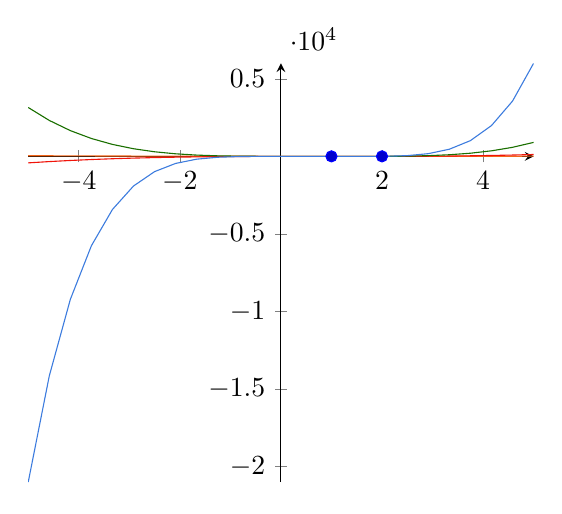
\begin{tikzpicture}
        \begin{axis}[axis x line=middle, axis y line=middle]
            \addplot coordinates {(1,0)(2,0)};
            \addplot[color=ocre] {(x-1)*(x-2)};
            \addplot [color=Red]{(2*x)*(x-1)*(x-2)};
            \addplot [color=deepGreen]{3*(x^2)*(x-1)*(x-2)};
            \addplot [color=deepBlue]{4*(x^3)*(x-1)*(x-2)};
        \end{axis}
    \end{tikzpicture}
    \end{align}
\end{document}